%! TeX program = lualatex
\documentclass{book}
\usepackage{graphicx}
\usepackage{amsthm}
\usepackage{amsmath,amssymb}
\usepackage{booktabs}
\usepackage[table]{xcolor}
\usepackage[utf8]{inputenc}
\usepackage[T1]{fontenc}
\usepackage[version=4]{mhchem}
\usepackage{stmaryrd}
\usepackage{graphicx}
\usepackage[export]{adjustbox}
\usepackage{caption}


\newtheorem{definition}{Definition}
\newtheorem{example}{Example}
\newtheorem{problem}{Problem}
\input{sym.tex}

\usepackage{comment}
\newif\ifsol
\definecolor{sol}{rgb}{0,0,1}\soltrue
%\definecolor{sol}{rgb}{1,1,1}\solfalse
\ifsol
  \newenvironment{sol}{\begingroup\color{sol}}{\endgroup}
\else
  \NewDocumentEnvironment{sol}{+b}{\vspace{2in}}{}
\fi

\begin{document}

\newcounter{marks}
\setcounter{marks}{0}

\chapter{Discrete Mathematics}
\section{Objectives}
Content adapted from \cite{piff1991discrete, rosen2007discrete, ldkr-ml2017-SetTheory}. Please read first five chapters of \cite{piff1991discrete} and first two chapters of \cite{rosen2007discrete}.
\begin{enumerate}
\item Defining Propositional Logic.
\item Defining Predicate Logic.
\item Defining Set, function, or relation model, and interpret the associated operations.
\item Operations between sets, functions, and relations.
\item Constructing proofs.
\item Logical reasoning to solve a strategic problem.
\item Model a real-life industry application applying formal methods.
\end{enumerate}

\section{Proposition Logic}
\begin{definition}[Proposition]
  A proposition is a statement that is either true or false.
\end{definition}

\subsection{Examples of propositions}
\begin{enumerate}
  \item Blue is a color.
  \item $1 + 1 = 2$.
  \item Any two primes have a common factor.
\end{enumerate}

\subsection{Examples of sentences that are not propositions}
\begin{enumerate}
  \item What is the color of sky?
  \item $1 + 1$.
  \item This sentence is false.
  \item $x^2 = x$.
  \item There exists an $x$ such that, $x^2 = x$.
  \item For all integers $x$, $x^2 = x$.
\end{enumerate}

\begin{definition}[Propositional variables]
  A proposition or a boolean variable is a variable that is either true or false.
\end{definition}

\begin{example}
  The following symbolic sentence is read as $x$ squared is equal to $y$.
$$ P(x, y) := x^2 = y $$.
This is not a proposition. 

However, for a given $x$ and $y$, the sentence becomes a proposition.
$$P(x=1, y=1) := 1^2 = 1$$
\end{example}

\section{Propositional calculus aka Boolean Algebra}

In propositional calculus, we have different names for Boolean algebra operators.

\begin{tabular}{ll}
  \toprule
  Boolean algebra & Propositional calculus \\
  \midrule
  OR gate $x + y$ & Disjunction: $P \lor Q$ \\
  AND gate $x \cdot y$ & Conjunction: $P \land Q$ \\
  NOT gate $\bar{y}$ & Negation: $\lnot P$ \\
  \bottomrule
\end{tabular}

\subsection{Implication $\implies$, $\supset$, $\rightarrow$ }

$$ (P \rightarrow Q) \equiv ((\neg P) \lor Q)$$

\subsection{Equivalence $\equiv$, $\leftrightarrow$}
$$ P \equiv Q = $$


\section{Propositional logic language}
\begin{definition}{Propositional alphabet}
  \begin{description}
    \item[Logic symbols] $\neg, \land, \lor, \supset, \equiv$
    \item[Propositional variables] $p \in \calP$
    \item[Separator symbols] "("  and ")"
  \end{description}
\end{definition}


\begin{definition}{Well formed formulas}
  \begin{itemize}
    \item every $p \in \calP$ is an atomic formula
    \item if A and B are formulas then $\neg A, A  \land B, A \lor B, A \supset B$ and $A \equiv B$ are formulas.
  \end{itemize}
\end{definition}

\begin{example}
Let’s consider a propositional language where p means ”Paola is happy”, q means
”Paola paints a picture”, and r means ”Renzo is happy”.
Formalize the following sentences:
\begin{enumerate}
  \item ”if Paola is happy and paints a picture then Renzo isn’t happy”
  \item ”if Paola is happy, then she paints a picture”
\item ”Paola is happy only if she paints a picture”
\end{enumerate}
The precision of formal languages avoid the ambiguities of natural
languages.
\end{example}

\begin{definition}
A Propositional interpretation is a function $I : P \to \{True,False\}$. (Evaluation of the formula with each variable set to true or false.)
\end{definition}

\begin{definition}
A formula A is\\
Valid if for all interpretations I , $I  \models  A$\\
Satisfiable if there is an interpretations I s.t., $I\models A$\\
Unsatisfiable if for no interpretations I , $I \models A$\\
\end{definition}

Propositional logic is an instrument for writing proofs. There are two connectives between two consecutive statements.
\subsection{Equivalence $\iff$}



\begin{example}[\cite{ldkr-ml2014-ExercisesBooklet}]
  Socrate says:\\
“If I’m guilty, I must be punished;
I must not be punished. Thus I’m not guilty.”\\
Is the argument logically correct?
\end{example}
\vspace{2in}

\begin{example}[\cite{ldkr-ml2014-ExercisesBooklet}]
  Socrate says:\\
“If I’m guilty, I must be punished;
I must be punished. Thus I’m guilty.”
Is the argument logically correct?
\end{example}
\vspace{2in}

\begin{example}
As a reward for saving his daughter from pirates, the King has given you the opportunity to win
a treasure hidden inside one of three trunks. The two trunks that do not hold the treasure are
empty. To win, you must select the correct trunk. Trunks 1 and 2 are each inscribed with the
message “This trunk is empty,” and Trunk 3 is inscribed with the message “The treasure is in
Trunk 2.” The Queen, who never lies, tells you that only one of these inscriptions is true, while
the other two are wrong. Which trunk should you select to win?
\label{ex:pirates}
\end{example}
\vspace{2in}

\begin{problem}(20 marks\addtocounter{marks}{20})
  Suppose that in Example~\ref{ex:pirates}, the inscriptions on Trunks 1,
2, and 3 are “The treasure is in Trunk 3,” “The treasure is
in Trunk 1,” and “This trunk is empty.” For each of these
statements, determine whether the Queen who never
lies could state this, and if so, which trunk the treasure
is in.\\
a) “All the inscriptions are false.”\\
b) “Exactly one of the inscriptions is true.”\\
c) “Exactly two of the inscriptions are true.”\\
d) “All three inscriptions are true.”\\
\end{problem}

\begin{sol}
Let $T_1$ denote that "Treasure is in Trunk 1", $T_2$ denote "Treasure is in
Trunk 2", $T_3$ denote "Treasure is in Trunk 3."

\noindent 
The inscription on Trunk 1 says: $I_1 = T_3$.\\
The inscription on Trunk 2 says: $I_2 = T_1$. \\
The inscription on Trunk 3 says: $I_3 = \overline{T_3}$.

\noindent 
a) "All the inscriptions are false" 
$= \overline{T_3} \cdot \overline{T_1} \cdot T_3 = \text{False}$. Hence, the Queen cannot say "a)".

\noindent 
b) "Exactly one of the inscriptions is true"
\begin{align*}
  &= I_1 \cdot \overline{I_2} \cdot \overline{I_3} + 
  \overline{I_1} \cdot {I_2} \cdot \overline{I_3} + 
  \overline{I_1} \cdot \overline{I_2} \cdot {I_3} \\
&= T_3 \cdot \overline{T_1} \cdot {T_3} + \overline{T_3} \cdot T_1 \cdot {T_3} 
+ \overline{T_3} \cdot \overline{T_1} \cdot \overline{T_3}\\
&= T_3 \cdot \overline{T_1} + 0
+ \overline{T_3} \cdot \overline{T_1} \\
&=(T_3 + \overline{T_3}) \overline{T_1} = \overline{T_1}
\end{align*}
The Queen who never lies can say "b)" if Trunk 1 does not contain the treasure.


\noindent 
b) "Exactly two of the inscriptions are true" = "Exact one of the inscriptions is false" =

\begin{align*}
  &= \overline{I_1} \cdot {I_2} \cdot {I_3} + 
  {I_1} \cdot \overline{I_2} \cdot {I_3} + 
  {I_1} \cdot {I_2} \cdot \overline{I_3} \\
  &= \overline{T_3} \cdot {T_1} \cdot \overline{T_3} 
  + {T_3} \cdot \overline{T_1} \cdot \overline{T_3} 
  + {T_3} \cdot {T_1} \cdot {T_3}\\
  &= \overline{T_3} \cdot {T_1} + 0
  + {T_3} \cdot {T_1} \\
  &=(\overline{T_3} + T_3) {T_1} = {T_1}
\end{align*}
The Queen who never lies can say "c)" if the Trunk 1 contains the treasure.


\noindent 
d) "All three inscriptions are true" = $T_3 \cdot T_1 \cdot \overline{T_3} = 0 $ = False. Hence the Queen can never say "d)".


\end{sol}


\begin{problem}[\cite{ldkr-ml2014-ExercisesBooklet}](20 marks\addtocounter{marks}{20})
Kyle, Neal, and Grant find themselves trapped in a dark and cold dungeon
(HOW they arrived there is another story). After a quick search the boys find
three doors, the first one red, the second one blue, and the third one green.
Behind one of the doors is a path to freedom. Behind the other two doors,
however, is an evil fire-breathing dragon. Opening a door to the dragon means
almost certain death.

On each door there is an inscription:
\bgroup
\def\arraystretch{1.5}
\begin{tabular}{|p{0.5in}|p{0.5in}|p{0.5in}|}
  \hline
  \cellcolor{red!25}freedom is behind this door
 & \cellcolor{blue!25}freedom is not behind this door
 & \cellcolor{green!25}freedom is not behind the blue door\\
  \hline
\end{tabular}
\egroup

Given the fact that at LEAST ONE of the three statements on the three doors
is true and at LEAST ONE of them is false, which door would lead the boys to
safety?
\end{problem}
\begin{sol}
\textbf{Language}
\begin{itemize}
  \item $r$ : "freedom is behind the red door"
  \item $b$ : "freedom is behind the blue door"
  \item $g$ : "freedom is behind the green door"
\end{itemize}

\textbf{Axioms}
\begin{enumerate}
  \item "behind one of the door is a path to freedom, behind the other two doors is an evil dragon"


\begin{equation*}
(r \wedge \neg b \wedge \neg g) \vee(\neg r \wedge b \wedge \neg g) \vee(\neg r \wedge \neg b \wedge g) \tag{2.4}
\end{equation*}


  \item "at least one of the three statements is true"


\begin{equation*}
r \vee \neg b \tag{2.5}
\end{equation*}


  \item "at least one of the three statements is false"


\begin{equation*}
\neg r \vee b \tag{2.6}
\end{equation*}
\end{enumerate}


\textbf{Solution}
\begin{center}
\begin{tabular}{|c|c|c||c|c|c|}
\hline
$r$ & $b$ & $g$ & 2.5 & 2.6 & 2.5 $\wedge 2.6$ \\
\hline\hline
$T$ & $F$ & $F$ & $T$ & $F$ & $F$ \\
$F$ & $T$ & $F$ & $F$ & $T$ & $F$ \\
$F$ & $F$ & $T$ & $T$ & $T$ & $T$ \\
\hline
\end{tabular}
\end{center}

Freedom is behind the green door!
\end{sol}


\section{Predicates}
\begin{definition}[Predicates]
  A predicate is a statement $P(x_1, \dots, x_n)$ involving $n$ (not necessarily boolean) variables $x_1 \in \calX_1$, $x_n \in \calX_n$, and which evaluates to a proposition $P(x_1, \dots, x_n) \in \{\text{True}, \text{False}\}$.
\end{definition}

\begin{example}
Let P(x) denote the statement “x > 3.” What are the truth values of P(4) and P(2)?
\end{example}

\subsection{Quantifiers}

\begin{definition}[Universal quantifier $\forall$]
\end{definition}

\begin{definition}[Existential quantifier $\exists$]
\end{definition}

\begin{example}
Let Q(x) be the statement “x < 2.” What is the truth value of the quantification $\forall x Q(x)$, where
the domain consists of all real numbers?
\end{example}

\begin{example}
Let Q(x) denote the statement “x = x + 1.” What is the truth value of the quantification $\exists xQ(x)$,
where the domain consists of all real numbers?
\end{example}

\subsection{Rules of Inference for Propositional Logic}
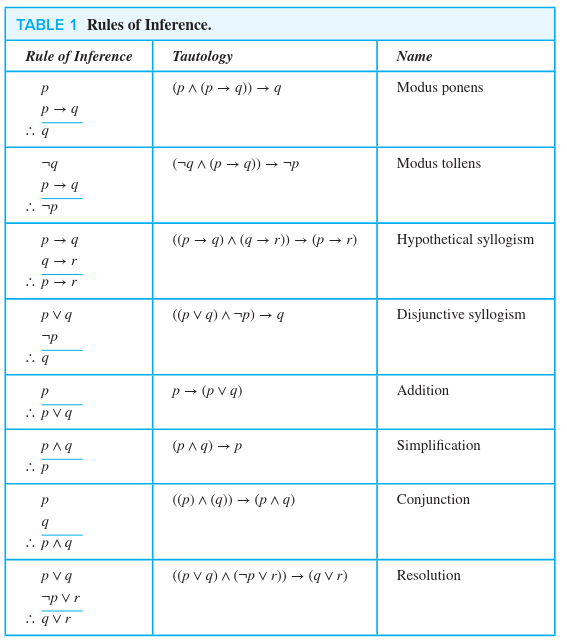
\includegraphics[width=0.7\linewidth]{imgs/rules-of-inference.png}


\begin{example}
Give a direct proof of the theorem “If n is an odd integer, then $n^2$ is odd.”
\end{example}
\vspace{4in}

\section{Sets}
The concept of \emph{set} is considered a primitive concept in math

A set is a collection of \emph{elements} whose description must be
unambiguous and unique: it must be possible to decide whether an
element belongs to the set or not.
\subsection{Describing sets}
\begin{description}
  \item[Listing]
  \item[Abstraction]
  \item[Eulero-Venn Diagrams]
\end{description}

\subsection{Russell's paradox}
{\color{sol}
Let R be the set of all sets that are not members of themselves (sometimes called "the Russell set"). If R is not a member of itself, then its definition entails that it is a member of itself; yet, if it is a member of itself, then it is not a member of itself, since it is the set of all sets that are not members of themselves. The resulting contradiction is Russell's paradox. In symbols:
}

    $$ R=\{x\mid x\not \in x\}.Then {R\in R\iff R\not \in R.}$$

\subsection{Relationships between sets}
\begin{definition}[Empty Set $\emptyset$]
  $\emptyset = \{  \}$
\end{definition}

\begin{definition}[Singleton $\{ a \}$]
  $A = \{a\}$ is singleton and $\{ a \} \neq a$.
\end{definition}

\begin{definition}[Set membership $a \in A$]
  $A = \{a, b, c\} \implies a \in A$ and $d \notin A$
\end{definition}

\begin{definition}[Set equality $A=B$]
  $A = \{a, b, c\}$ $B=\{c, b, a, a\}$ $\implies A=B$.
\end{definition}

\begin{definition}[Subset $A\subseteq B$]
  $A = \{a, b, c\}$ $B=\{c, b, a, a\}$ $\implies A\subseteq B$.\\
  $A = \{a, b, c\}$ $B=\{c, b, a, a, d\}$ $\implies A\subseteq B$.
\end{definition}

\begin{definition}[Subset $A\subset B$]
  $A = \{a, b, c\}$ $B=\{c, b, a, a, d\}$ $\implies A\subset B$.
  $A = \{a, b, c\}$ $B=\{c, b, a, a\}$ $\implies A \not\subset B$.\\
\end{definition}

\begin{definition}[Power set $P(A)$, $2^A$]
  $A = \{a,b, c\}$, then $P(A) = \{\emptyset, \{a\}, \{b\}, \{c\}, \{a, b\}, \{b, c\}, \{a, c\}, \{a, b, c\}$.
\end{definition}

\begin{definition}[Union of two sets $A\cup B$]
  $A = \{a, b, c\}$ $B=\{c, b, a, a, d\}$ $\implies A\cup B = \{a, b, c, d\}$.
\end{definition}

\begin{definition}[Intersection of two sets $A\cap B$]
  $A = \{a, b, c\}$ $B=\{c, b, a, a, d\}$ $\implies A\cap B = \{a, b, c\}$.
\end{definition}

\begin{definition}[Set difference $A\setminus B$, $A-B$]
  $A = \{a, b, c\}$ $B=\{c, b, a, a, d\}$ $\implies A\setminus B = A-B = \{\} = \emptyset$.\\
  $B\setminus A = B-A = \{d\}$.\\
\end{definition}

\begin{definition}[Set complement $\bar{A}$, $C_UA$]
  Given a universal set $U$, complement is defined as $\bar{A} = C_U A= U - A$. Also, $A \cup \bar{A} = U$.
\end{definition}


\begin{example}
  Prove that  $U = (A\cap B) \cup \overline{(A\cap B)}$
\end{example}

\begin{example}
  $A=\{a,e,i,o,\{u\}\}$ and $B = \{i, o,  u\}$
  \begin{enumerate}
    \item $B  \in A$
    \item $(B - \{i, o\}) \in  A$
    \item $\{a\} \cup \{i\} \subset A$
    \item $\{u\} \in A$
    \item $\{\{u\}\} \in  A$
    \item $B - A =  \emptyset$
    \item $i \in A \cap B$
    \item $\{i, o\} = A\cap B$
  \end{enumerate}
\end{example}

\begin{example}
  Prove De Morgan laws for sets $\overline{A \cap B} = \bar{A} \cup \bar{B}$, and $\overline{A \cup B} = \bar{A} \cap \bar{B}$.
\end{example}



\bibliography{main}
\bibliographystyle{plainnat}

Total marks: \arabic{marks}
\newpage



\section{Relations}

\begin{definition}[Cartesian product of sets $A \times B$]
  $A \times B =  \{(a, b):  \forall a  \in  A, \forall b \in B\}$
\end{definition}

\begin{definition}[Relation $R \subseteq A \times B$]
We write $a R y$ to read as "a  is R-related to b".
\end{definition}
\begin{example}
given $A = \{3, 5, 7\}$, $B = {2, 4, 6, 8, 10, 12}$ and $aRb$ iff a is a
divisor of b, then $R = \{(3, 6), (3, 12), (5, 10)\}$
\end{example}


\begin{definition}[Domain of $R$]
$$\text{dom}(R) = \{ a \in A : \exists y \in B (a R y) \}$$
\end{definition}

\begin{definition}[Image/Range of $R$]
$$\text{Range}(R) = \text{Im}(R) = \{ b \in B : \exists x \in A (x R b) \}$$
\end{definition}

\begin{definition}[Inverse of $R$]
  $$R^{-1} = \{(b, a) | (a R b)\}$$
\end{definition}

\section{Functions}

\begin{definition}[Function $f: A \to B$]
Given two sets A and B, a function f from A to B is a relation
that associates to each element a in A exactly one element b in B.
Denoted with\\
$f : A \to B$

\end{definition}

\subsection{Classes of Functions}
\begin{definition}[Surjective]
  {\color{sol} If $b \in B$, then $\exists a \in A|f(a) = b$}
\end{definition}

\begin{definition}[Injective]
  {\color{sol} If $f(a_1) = f(a_2)B$, only if $a_1 = a_2$}
\end{definition}

\begin{definition}[Bijective]
  Both Surjective and Bijective
\end{definition}

\begin{definition}[Inverse]
  {\color{sol} $f^{-1} : B \to A$ exists if $f$ is Bijective. $f^{-1}(b) = a$ if and only if $f(a) = b$.}
\end{definition}

\begin{definition}[Composition]
  $f: A \to B$, $g : B \to C$. $g \circ f : A \to C$; $(g \circ f)(a) = g(f(a))$
\end{definition}

\newpage
\section{More exercises}

\begin{example}
Define an appropriate language and formalize the following sentences using
First Order Logic formulas.\\
\begin{enumerate}
\item Bill has at least one sister.
\item Bill has no sister.
\item Bill has at most one sister.
\item Bill has (exactly) one sister.
\item Bill has at least two sisters.
\item Every student takes at least one course.
\item Only one student failed Geometry.
\item No student failed Geometry but at least one student failed Analysis.
\item Every student who takes Analysis also takes Geometry.
\end{enumerate}
\end{example}

{\color{sol}
  \begin{enumerate}
\item $\exists x.SisterOf (x, Bill)$
\item $\neg \exists x.SisterOf (x, Bill)$
\item $\forall x\forall y.(SisterOf (x, Bill) \land  SisterOf (y, Bill) \rightarrow x = y)$
\item $\exists x.(SisterOf (x, Bill) \land  \forall y.(SisterOf (y, Bill) \rightarrow x = y))$
\item $\exists x\exists y.(SisterOf (x, Bill) \land  SisterOf (y, Bill) \land  \neg (x = y))$
\item $\forall x.(Student(x) \rightarrow \exists y.(Course(y) \land  T akes(x, y)))$
\item $\exists x.(Student(x)\land F ailed(x, Geometry)\land \forall y.(Student(y)\land F ailed(y, Geometry) →$
\item=$ y))$
\item $\neg \exists x.(Student(x)\land F ailed(x, Geometry))\land \exists x.(Student(x)\land F ailed(x, Analysis))$
\item $\forall x.(Student(x) \land  Takes(x, Analysis) \rightarrow Takes(x, Geometry))$
  \end{enumerate}
}

\begin{example}%{Exercise 3.14.}
Consider the following sentences:

\begin{enumerate}
  \item All actors and journalists invited to the party are late.
  \item There is at least a person who is on time.
  \item There is at least an invited person who is neither a journalist nor an actor.
\end{enumerate}

Formalize the sentences and prove that 3. is not a logical consequence of 1 . and 2.

{\color{sol}
\textbf{Solution.}
\begin{enumerate}
  \item $\quad \forall x \cdot((a(x) \vee j(x)) \wedge i(x) \rightarrow l(x))$
  \item $\quad \exists x . \neg l(x)$
  \item $\quad \exists x .(i(x) \wedge \neg a(x) \wedge \neg j(x))$
\end{enumerate}

It's sufficient to find an interpretation $\mathcal{I}$ for which the logical consequence does not hold:

\begin{center}
\begin{tabular}{|c|c|c|c|c|}
\hline
 & $l(x)$ & $a(x)$ & $j(x)$ & $i(x)$ \\
\hline\hline
Bob & $F$ & $T$ & $F$ & $F$ \\
Tom & $T$ & $T$ & $F$ & $T$ \\
Mary & $T$ & $F$ & $T$ & $T$ \\
\hline
\end{tabular}
\end{center}
}

\end{example}


% \begin{example}%Exercise 3.16.\\
% Provide a FOL language and a set of axioms that formalize the graph coloring problem of a graph with at most $n$ nodes, with connection degree $\leq m$, and with less then $k+1$ colors.
% 
% \begin{itemize}
%   \item node degree: number of adjacent nodes
%   \item connection degree of a graph: max among all the degree of its nodes
%   \item graph coloring problem: given a non-oriented graph, associate a color to each of its nodes in such a way that no pair of adjacent nodes have the same color.
% \end{itemize}
% \end{example}
% 
% {\color{sol}
% \textbf{Solution.}
% %\section{First Order Logic}
% %\section{Language}
% \begin{itemize}
%   \item A unary function color, where color $(x)$ is the color associated to the node x
%   \item A unary predicate node, where node $(x)$ means that $x$ is a node
%   \item A binary predicate edge, where edge $(x, y)$ means that $x$ is connected to $y$
% \end{itemize}
% 
% %\section{Axioms}
% \begin{enumerate}
%   \item $\forall x \forall y .(\operatorname{edge}(x, y) \rightarrow(\operatorname{color}(x) \neq \operatorname{color}(y))$\\
% "Two connected node are not equally colored."
%   \item $\forall x \forall x_{1} \ldots \forall x_{k+1} \cdot\left(\bigwedge_{h=1}^{k+1} \operatorname{edge}\left(x, x_{h}\right) \rightarrow \bigvee_{i, j=1, j \neq i}^{k+1} x_{i}=x_{j}\right)$\\
% "A node does not have more than $k$ connected nodes."
% \end{enumerate}
% }

%   \item 
%     $$\forall x \forall y . (\text{edge}(x,y) \rightarrow (\text{color}(x) \ne \text{color}(y)))$$
%     "Two connected node are not equally colored"
%   \item
%     $$ \forall x \forall x_1 \dots \forall x_{k+1} .
%     \left(\bigwedge\limits_{h=1}^{k+1} \text{edge}(x, x_h) \rightarrow \bigvee\limits_{i=1}^{k+1}\bigvee\limits_{j=1,j\ne i}^{k+1} x_i = x_j \right)
%     $$
%     "A node does not have more than $k$ connected nodes"

\begin{example} % {Exercise 3.17.}
Let $\left\{c_{1}, . ., c_{k}\right\}$ be a non empty and finite set of colors. A partially colored directed graph is a structure $\langle N, R, C\rangle$ where

\begin{itemize}
  \item $N$ is a non empty set of nodes
  \item R is a binary relation on $N$
  \item $C$ associates colors to nodes (not all the nodes are necessarily colored,. and each node has at most one color)
\end{itemize}

Provide a first order language and a set of axioms that formalize partially colored graphs. Show that every model of this theory correspond to a partially colored graph, and vice-versa. For each of the following properties, write a formula which is true in all and only the graphs that satisfies the property:

\begin{enumerate}
  \item connected nodes don't have the same color
  \item the graph contains only 2 yellow nodes
  \item starting from a red node one can reach in at most 4 steps a green node
  \item for each color there is at least a node with this color
  \item the graph is composed of $|C|$ disjoint non empty subgraphs, one for each color
\end{enumerate}

\end{example}
\begin{sol}
\textbf{Solution.}
\textbf{Language}
\begin{itemize}
  \item a binary predicate edge, where edge( $n, m$ ) means that node $n$ is connected to node $m$.
  \item a binary predicate color, where color($n, x$ ) means that node $n$ has color $x$
  \item the following constants: yellow, green,red
\end{itemize}

\textbf{Axioms}
\begin{enumerate}
  \item
    "each node has at most one color"
    $$\forall n \forall x . (\text{color}(n, x) \rightarrow \neg \exists y. (y \ne x \land \text{color}(n, y)))$$
\end{enumerate}

\textbf{Formulae}
$$
\forall n \forall x .(\operatorname{color}(n, x) \rightarrow \neg \exists y .(y \neq x \wedge \operatorname{color}(n, y)))
$$

\begin{enumerate}
  \item "connected nodes do not have the same color"
\end{enumerate}

$$
\forall n \forall m \forall x .(\operatorname{edge}(n, m) \wedge \operatorname{color}(n, x) \rightarrow \neg \operatorname{color}(m, x))
$$

\begin{enumerate}
  \setcounter{enumi}{1}
  \item "the graph contains only two yellow nodes"
\end{enumerate}

$$
\begin{array}{r}
\exists n \exists n^{\prime} .\left(\text { color }(n, \text { yellow }) \wedge \text { color }\left(n^{\prime}, \text { yellow }\right) \wedge n \neq n^{\prime} \wedge\right. \\
\left.\forall m .\left(m \neq n \wedge m \neq n^{\prime} \rightarrow \neg \operatorname{color}(m, \text { yellow })\right)\right)
\end{array}
$$

\begin{enumerate}
  \setcounter{enumi}{2}
  \item "starting from a red node one can reach in at most 4 steps a green node"
\end{enumerate}

$$
\begin{aligned}
& \forall n(\text { color }(n, \text { red }) \rightarrow \\
& \left(\exists n_{1} \cdot\left(\text { edge }\left(n, n_{1}\right) \wedge \text { color }\left(n_{1}, \text { green }\right)\right) \vee\right. \\
& \exists n_{1}, n_{2} \cdot\left(\text { edge }\left(n, n_{1}\right) \wedge \text { edge }\left(n_{1}, n_{2}\right) \wedge \text { color }\left(n_{2}, \text { green }\right)\right) \vee \\
& \exists n_{1}, n_{2}, n_{3} \cdot\left(\text { edge }\left(n, n_{1}\right) \wedge \text { edge }\left(n_{1}, n_{2}\right) \wedge \text { edge }\left(n_{2}, n_{3}\right) \wedge \operatorname{color}\left(n_{3}, \text { green }\right)\right) \vee \\
& \exists n_{1}, n_{2}, n_{3}, n_{4} \cdot\left(\text { edge }\left(n, n_{1}\right) \wedge \operatorname{edge}\left(n_{1}, n_{2}\right) \wedge \operatorname{edge}\left(n_{2}, n_{3}\right) \wedge \operatorname{edge}\left(n_{3}, n_{4}\right) \wedge \operatorname{color}\left(n_{4}, \text { green }\right)\right) \\
& ))
\end{aligned}
$$

\begin{enumerate}
  \setcounter{enumi}{3}
  \item "for each color there is at least a node with this color"
\end{enumerate}

$$
\forall x \exists n . \operatorname{color}(n, x)
$$

\begin{enumerate}
  \setcounter{enumi}{4}
  \item "the graph is composed of $|C|$ disjoint non empty subgraphs, one for each color"
\end{enumerate}

$$
\begin{aligned}
& \forall x \exists n . \operatorname{color}(n, x) \wedge \\
& \forall n \exists x . \operatorname{color}(n, x) \wedge \\
& \forall n \forall x .(\operatorname{color}(n, x) \rightarrow \neg \exists y .(y \neq x \wedge \operatorname{color}(n, y))) \wedge \\
& \forall n \forall m \forall x .(n \neq m \wedge \operatorname{color}(n, x) \wedge \operatorname{color}(m, x) \rightarrow \\
& \left.\left(\operatorname{edge}(n, m) \bigvee_{i=1}^{|N|}\left(\exists n_{1}, . ., n_{i} .\left(\operatorname{edge}\left(n, n_{1}\right) \bigwedge_{j=1}^{i-1} \operatorname{edge}\left(x_{j}, x_{j}+1\right) \wedge \operatorname{edge}\left(n_{i}, m\right)\right)\right)\right)\right)
\end{aligned}
$$
\end{sol}

\begin{problem}(40 marks\addtocounter{marks}{40}) % {Exercise 3.18.}
Minesweeper is a single-player computer game invented by Robert Donner in 1989. The object of the game is to clear a minefield without detonating a mine. The game screen consists of a rectangular field of squares. Each square can be cleared, or uncovered, by clicking on it. If a square that contains a mine is clicked, the game is over. If the square does not contain a mine, one of two things can happen: (1) A number between 1 and 8 appears indicating the amount of adjacent (including diagonally-adjacent) squares containing mines, or (2) no number appears; in which case there are no mines in the adjacent cells. An example of game situation is provided in the following figure:\\
Provide a first order language that allows to formalize the knowledge of a player in a game state. In such a language you should be able to formalize the following knowledge:

\begin{enumerate}
  \item there are exactly $n$ mines in the minefield
  \item if a cell contains the number 1 , then there is exactly one mine in the adjacent cells.
\end{enumerate}
%\begin{figure}[h]
%\begin{center}
  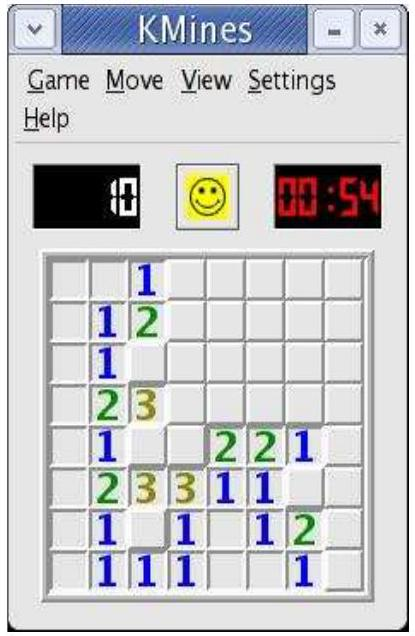
\includegraphics[alt={},max width=0.25\linewidth]{imgs/minesweeper.jpg}
%\captionsetup{labelformat=empty}
%\caption{Figure 3.1: An example of a state in the Mines game}
%\end{center}
%\end{figure}

\begin{enumerate}
  \setcounter{enumi}{2}
  \item show by means of deduction that there must be a mine in the position $(3,3)$ of the game state of picture 3.1
\end{enumerate}

Suggestion: define the predicate Adj( $x, y$ ) to formalize the fact that two cells $x$ and $y$ are adjacent

\end{problem}

\begin{sol}
\textbf{Solution.}
\textbf{Language}
\begin{enumerate}
  \item A unary predicate mine, where mine $(x)$ means that the cell xcontains a mine
  \item A binary predicate adj, where adj( $x, y$ ) means that the cell $x$ is adjacent to the cell $y$
  \item A binary predicate contains, where contains( $x, n$ ) means that the cell $x$ contains the number $n$
\end{enumerate}

\textbf{Axioms}
\begin{enumerate}
  \item There are exactly $n$ mines in the game.
\end{enumerate}

$$
\exists x_{1}, . . \exists x_{n}\left(\bigwedge_{i=1}^{n} \operatorname{mine}\left(x_{i}\right) \wedge \forall y\left(\operatorname{mine}(y) \rightarrow \bigvee_{i=1}^{n} y=x_{i}\right)\right)
$$

\begin{enumerate}
  \setcounter{enumi}{1}
  \item If a cell contains the number 1 , then there is exactly one mine in the adjacent cells.\\
$\forall x .(\operatorname{contains}(x, 1) \rightarrow \exists z .(\operatorname{adj}(x, z) \wedge \operatorname{mine}(z) \wedge \forall y .(\operatorname{adj}(x, y) \wedge \operatorname{mine}(y) \rightarrow y=z)))$
  \item Show by means of deduction that there must be a mine in the position $(3,3)$\\
from Picture 3.1 we have:\\
a. contains((2,2),1)\\
b. $\neg \operatorname{mine}((1,1)) \wedge \neg \operatorname{mine}((1,2)) \wedge \neg \operatorname{mine}((1,3))$\\
c. $\neg \operatorname{mine}((2,1)) \wedge \neg \operatorname{mine}((2,2)) \wedge \neg \operatorname{mine}((2,3))$\\
d. $\neg \operatorname{mine}((3,1)) \wedge \neg \operatorname{mine}((3,2))$\\
we can deduce:\\
e. $\exists z \cdot(\operatorname{adj}((2,2), z) \wedge \operatorname{mine}(z) \wedge \forall y \cdot(\operatorname{adj}((2,2), y) \wedge \operatorname{mine}(y) \rightarrow y=z)) \quad \rightsquigarrow$ from a. and axiom 2\\
f. mine $((1,1)) \vee \operatorname{mine}((1,2)) \vee \operatorname{mine}((1,3)) \vee \operatorname{mine}((2,1)) \vee \operatorname{mine}((2,2)) \vee \operatorname{mine}((2,3)) \vee \operatorname{mine}((3,1)) \vee \operatorname{mine}((3,2)) \vee \operatorname{mine}((3,3)) \rightsquigarrow$ from $e$.\\
g. mine $((3,3)) \quad \rightsquigarrow$ from b.,c.,d. and $f$.
\end{enumerate}

\begin{itemize}
  \item 
\end{itemize}
\end{sol}

\begin{problem}(40 marks\addtocounter{marks}{40})%{Exercise 3.19.}
Formalize in first order logic the train connections in Italy. Provide a language that allows to express the fact that a town is directly connected (no intermediate train stops) with another town, by a type of train (e.g., intercity, regional, interregional). Formalize the following facts by means of axioms:

\begin{enumerate}
  \item There is no direct connection from Rome to Trento
  \item There is an intercity from Rome to Trento that stops in Firenze, Bologna and Verona.
  \item Regional trains connect towns in the same region
  \item Intercity trains don't stops in small towns.
\end{enumerate}

\end{problem}
\begin{sol}{\color{sol}
\textbf{Solution}. We define the language as follows

Constants $RM, FI, BO, VR, TN, \ldots$ are identifiers of the towns of Roma, Firenze, Bologna, Verona, Trento, . . . and InterCity, Regional, . . . are the identifiers of the type of trains

Predicates Train with arity equal to 1 , where Train $(x)$ means $x$ is a train Town with arity equal to 1 , where Train $(x)$ means $x$ is a town\\
SmallTown with arity equal to 1, where Train $(x)$ means $x$ is a small town TrainType with arity equal to 2 , where TrainType $(x, y)$ means that the train $x$ is of type $y$.\\
IsInRegion with arity equal to 2 , where IsInRegion ( $x, y$ ) means that the town $x$ is in region $y$. DirectConn with arity equal to 3, where DirectConn $(x, y, z)$ means that the train $x$ directly connects (with no intermediated stops) the towns $y$ and $z$.

Background axioms With these set of axioms we have to formalize some background knowledge which is necessary to make the formalization more adeguate

\begin{enumerate}
  \item a train has exactly one train type;
\end{enumerate}


\begin{equation*}
\forall x(\operatorname{Train}(x) \rightarrow \exists y(\operatorname{TrainType}(x, y))) \wedge \forall x y z(\operatorname{TrainType}(x, y) \wedge \operatorname{TrainType}(x, z) \rightarrow y=z) \tag{3.1}
\end{equation*}


\begin{enumerate}
  \setcounter{enumi}{1}
  \item Intercity type is different from regional type:
\end{enumerate}


\begin{equation*}
\neg(\text { InterCity }=\text { Regional }) \quad(\text { also written as InterCity } \neq \text { Regional }) \tag{3.2}
\end{equation*}


\begin{enumerate}
  \setcounter{enumi}{2}
  \item A town is associated to exactly one region
\end{enumerate}


\begin{equation*}
\forall x(\operatorname{Town}(x) \rightarrow \exists y(\operatorname{IsInRegion}(x, y))) \wedge \forall x y z(\operatorname{IsInRegion}(x, y) \wedge \operatorname{IsInRegion}(x, z) \rightarrow y=z) \tag{3.3}
\end{equation*}
}\end{sol}

\end{document}
